\paragraph{4. Do the lost relations result in New Observable Behaviors?}

    To address this, we divide our cases into two parts; one for each type of relation lost:
    \begin{tasks}(2)
        \task $\reln{k}{hb}{e}$
        \task $\reln{e}{hb}{k}$
    \end{tasks}

    For the first case, we have the following possibilities:
    \begin{figure}[H]
        \centering
        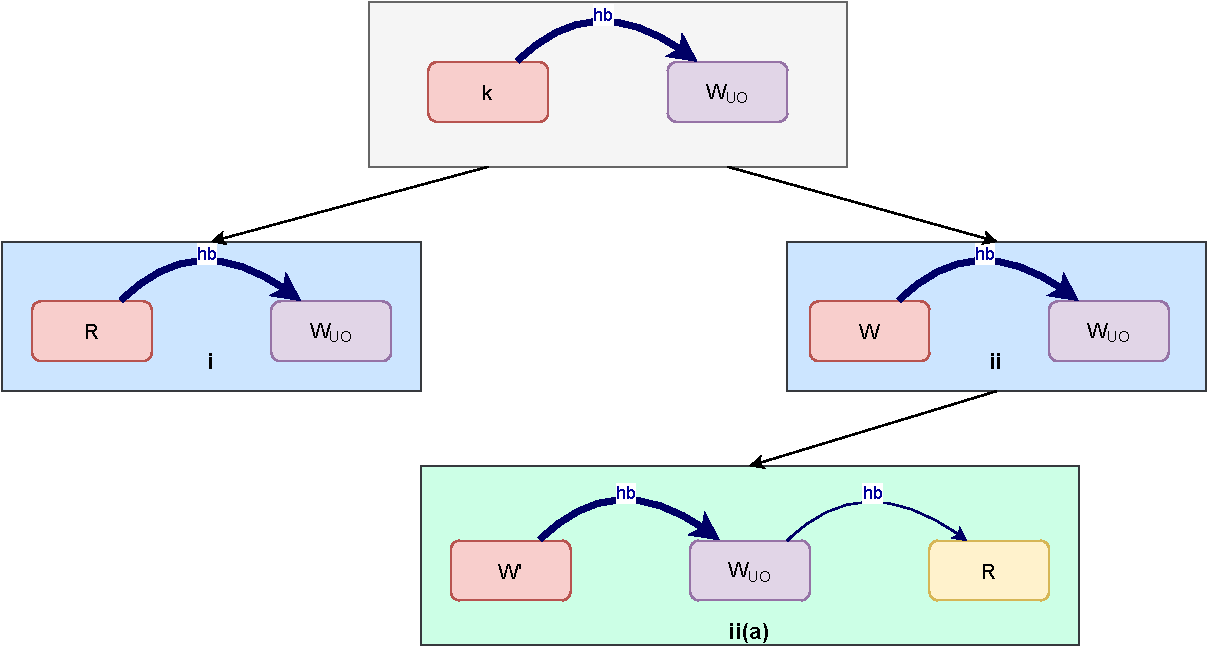
\includegraphics[scale=0.5]{Elimination/WriteElimProof/ProofParts/Part4Case1.pdf}
        \caption{First case possibilities (change caption stimiar to that for read elim)}
    \end{figure}

    We can observe the following:
    \begin{itemize}
        \item (i) is a pattern from Coherent Reads that restricts the read $R$ reading from $W$. And this will remain the case even after elimination of $W$.
        \item (ii)(a) is a pattern from Coherent reads, forbidding $R$ to read from some $W'$. This will remain the case after elimination of $W$ if firstly we have $\reln{d}{hb}{R}$. By Lemma 2 this is indeed the case. Secondly, we need to ensure that after elimination, the Coherent Reads pattern with $d$ now restricts the exact set of $\stck{_{rbf}}$  relations. Since we have no certain information on the range of $R$ or $W'$, we require the ranges of $e$ and $d$ to be same for our requirement to hold in general. 
        \item \textbf{PErhaps explain the above argument in more detail}
    \end{itemize}

    For the first case, we have the following possibilities:
    \begin{figure}[H]
        \centering
        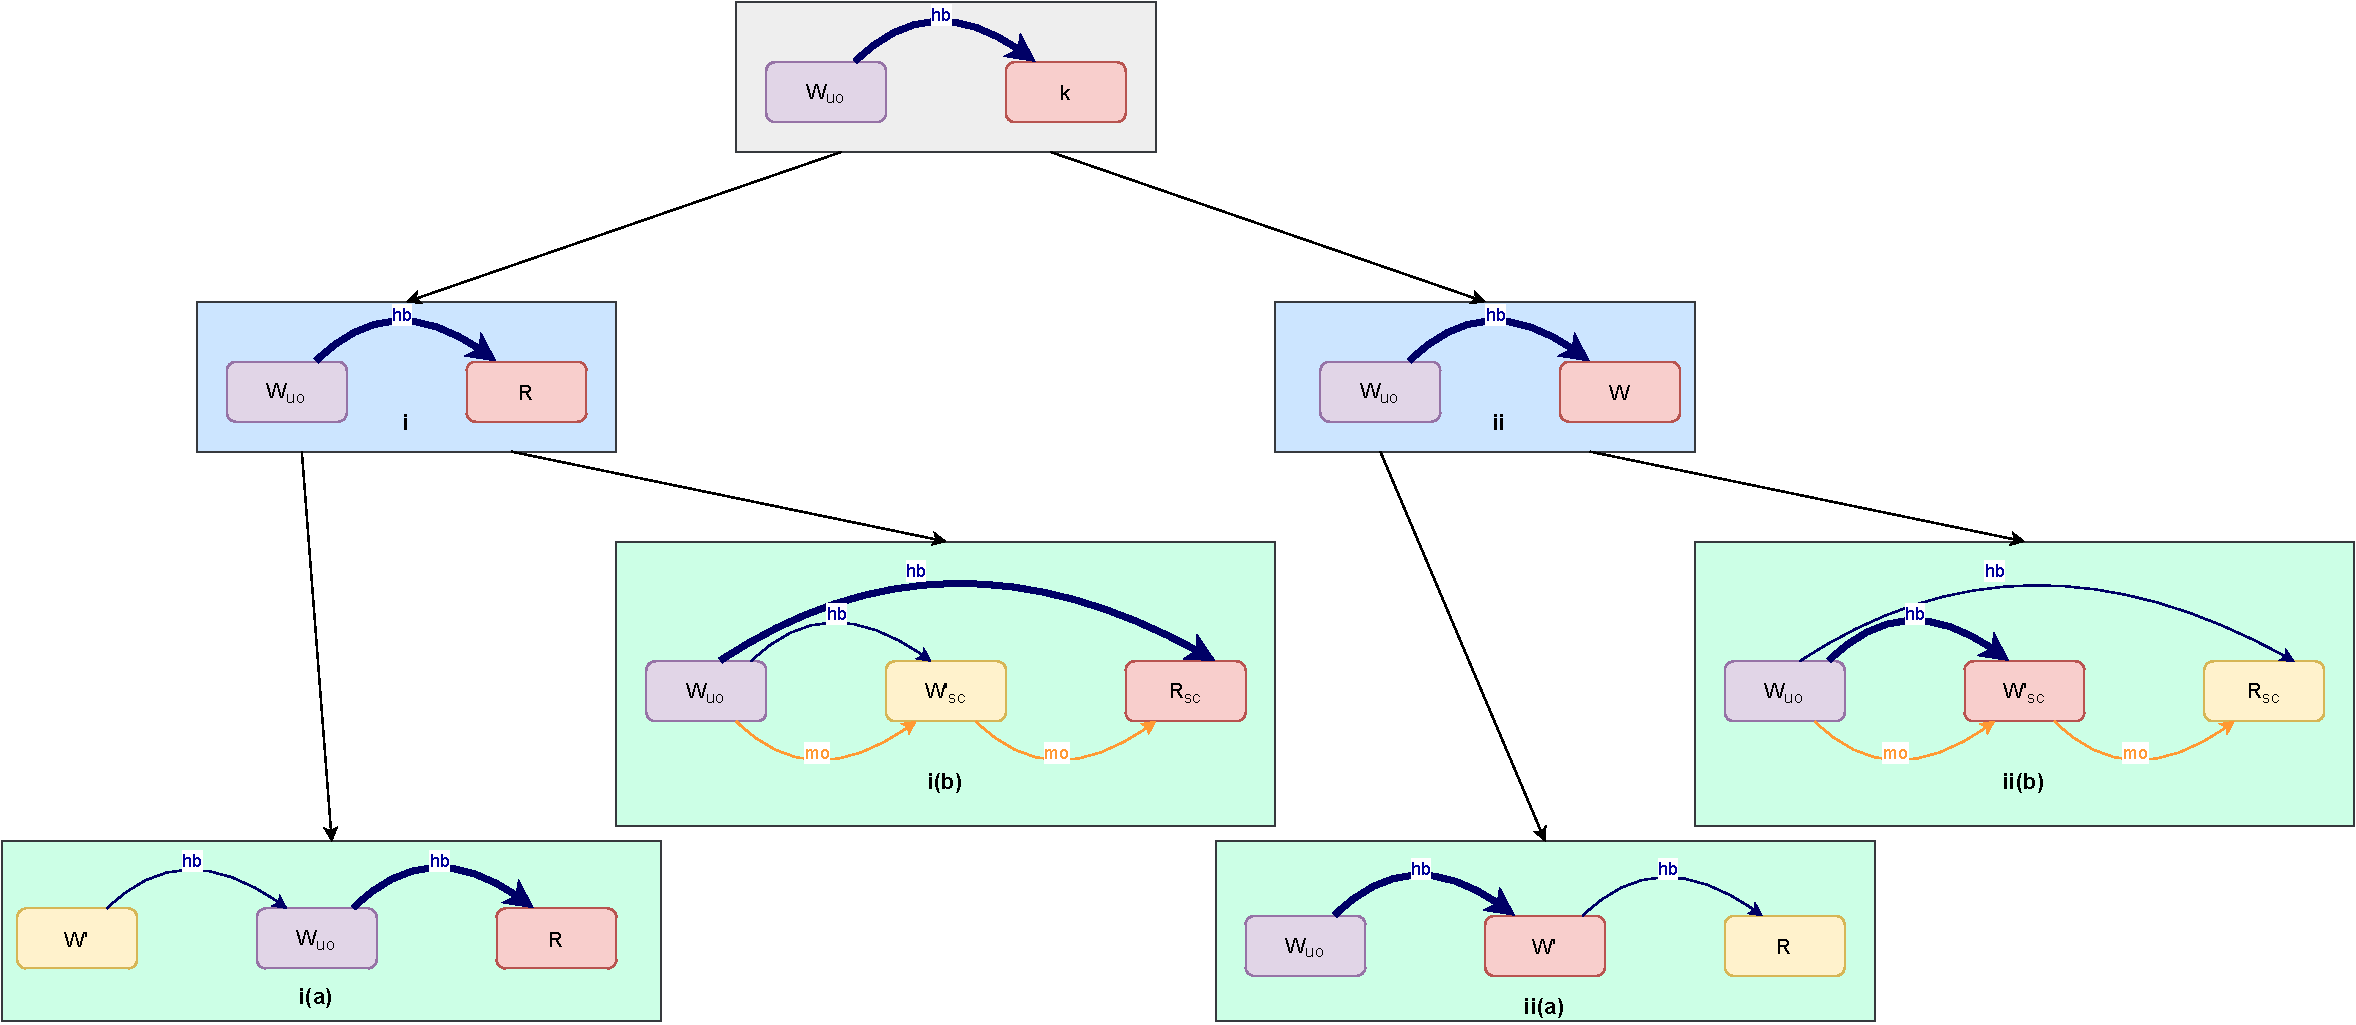
\includegraphics[scale=0.3]{Elimination/WriteElimProof/ProofParts/Part4Case2.pdf}
        \caption{Second case possibilities (change caption stimiar to that for read elim)}
    \end{figure}

    We make the following observations:
    \begin{itemize}
        \item (i)(a) has the similar argument to the previous case's (ii)(a), requiring $e$ and $d$ to have equal ranges.
        \item (i)(b) is a pattern of Sequentially Consistent Atomics, which restricts $R$ from reading anything of $W$. This will reamin the case after $W$ is eliminated. 
        \item (ii)(a) is a pattern of Coherent Reads, restricting $R$ from reading $W$. This will remain the case after eliminating $W$.
        \item (ii)(b) is the same as (i)(b), hence the argument remains the same.  
    \end{itemize}

    In all the above cases, observe that on keeping range of $e$ and $d$ equal, none of the patterns introduce any new observable behavior. Hence, if we have two consecutive writes of equal ranges, of which the first one has access mode unorderd, the set of Observable Behaviors without the write is a subset of that with it present. 